\subsubsection{UC13.1 -  Visualizzazione lista di tutte le funzioni}
\begin{figure}[H]
	\centering
	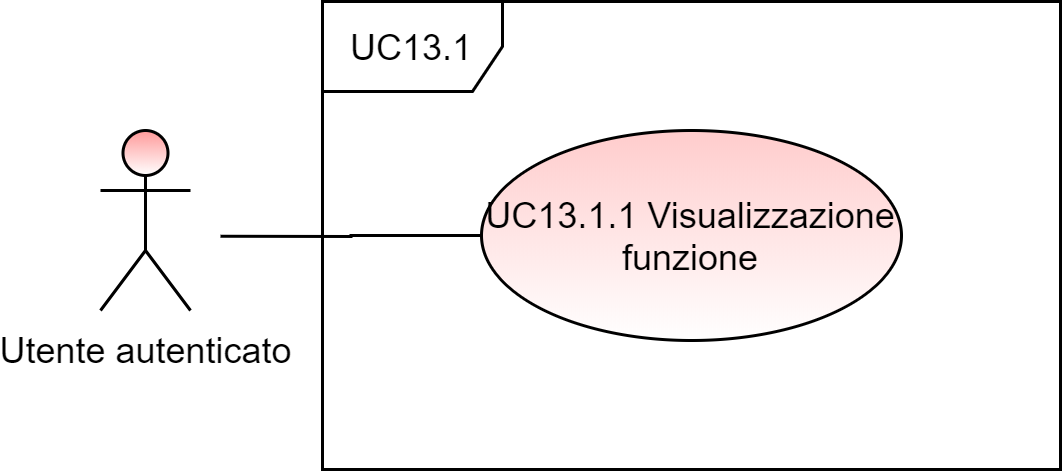
\includegraphics[scale=\ucs]{./res/img/UC13.1.png}
	\caption {UC13.1 -  Visualizzazione lista di tutte le funzioni}
\end{figure}
\begin{itemize}
	\item \textbf{Attori primari:} \ua{};
	\item \textbf{Descrizione:} l’utente richiede la visualizzazione della lista di tutte le funzioni fornite dal servizio eseguendo il comando list. Il sistema stampa a video tale lista; 
	\item \textbf{Scenario principale:} 
	\begin{itemize}
		\item l'utente inserisce correttamente ed esegue il comando \lista{}. 
		\item viene visualizzata la lista di tutte le funzioni disponibili presso il servizio;
	\end{itemize}
	\item \textbf{Estensioni:} 
	\begin{itemize}
		\item \textbf{UC13.3:} non è stata ancora pubblicata alcuna funzione, di conseguenza viene visualizzato un messaggio di avviso. 
	\end{itemize}
	\item \textbf{Precondizione:} l'utente inserisce correttamente ed esegue il comando \lista{};
	\item \textbf{Postcondizione:} la CLI\ped{\textit{G}} riporta la lista di tutte le funzioni fornite dal servizio.
\end{itemize}